We study the change of BDT output shape when varying the \CV/\Ct\ coupling scenario.
Figure~\ref{fig:bdtvscvct} shows the two BDT output shapes in the three lepton channel for five different values of \Ct, with \CV\ fixed at $1.0$.
\begin{figure} [!h]
  \centering
  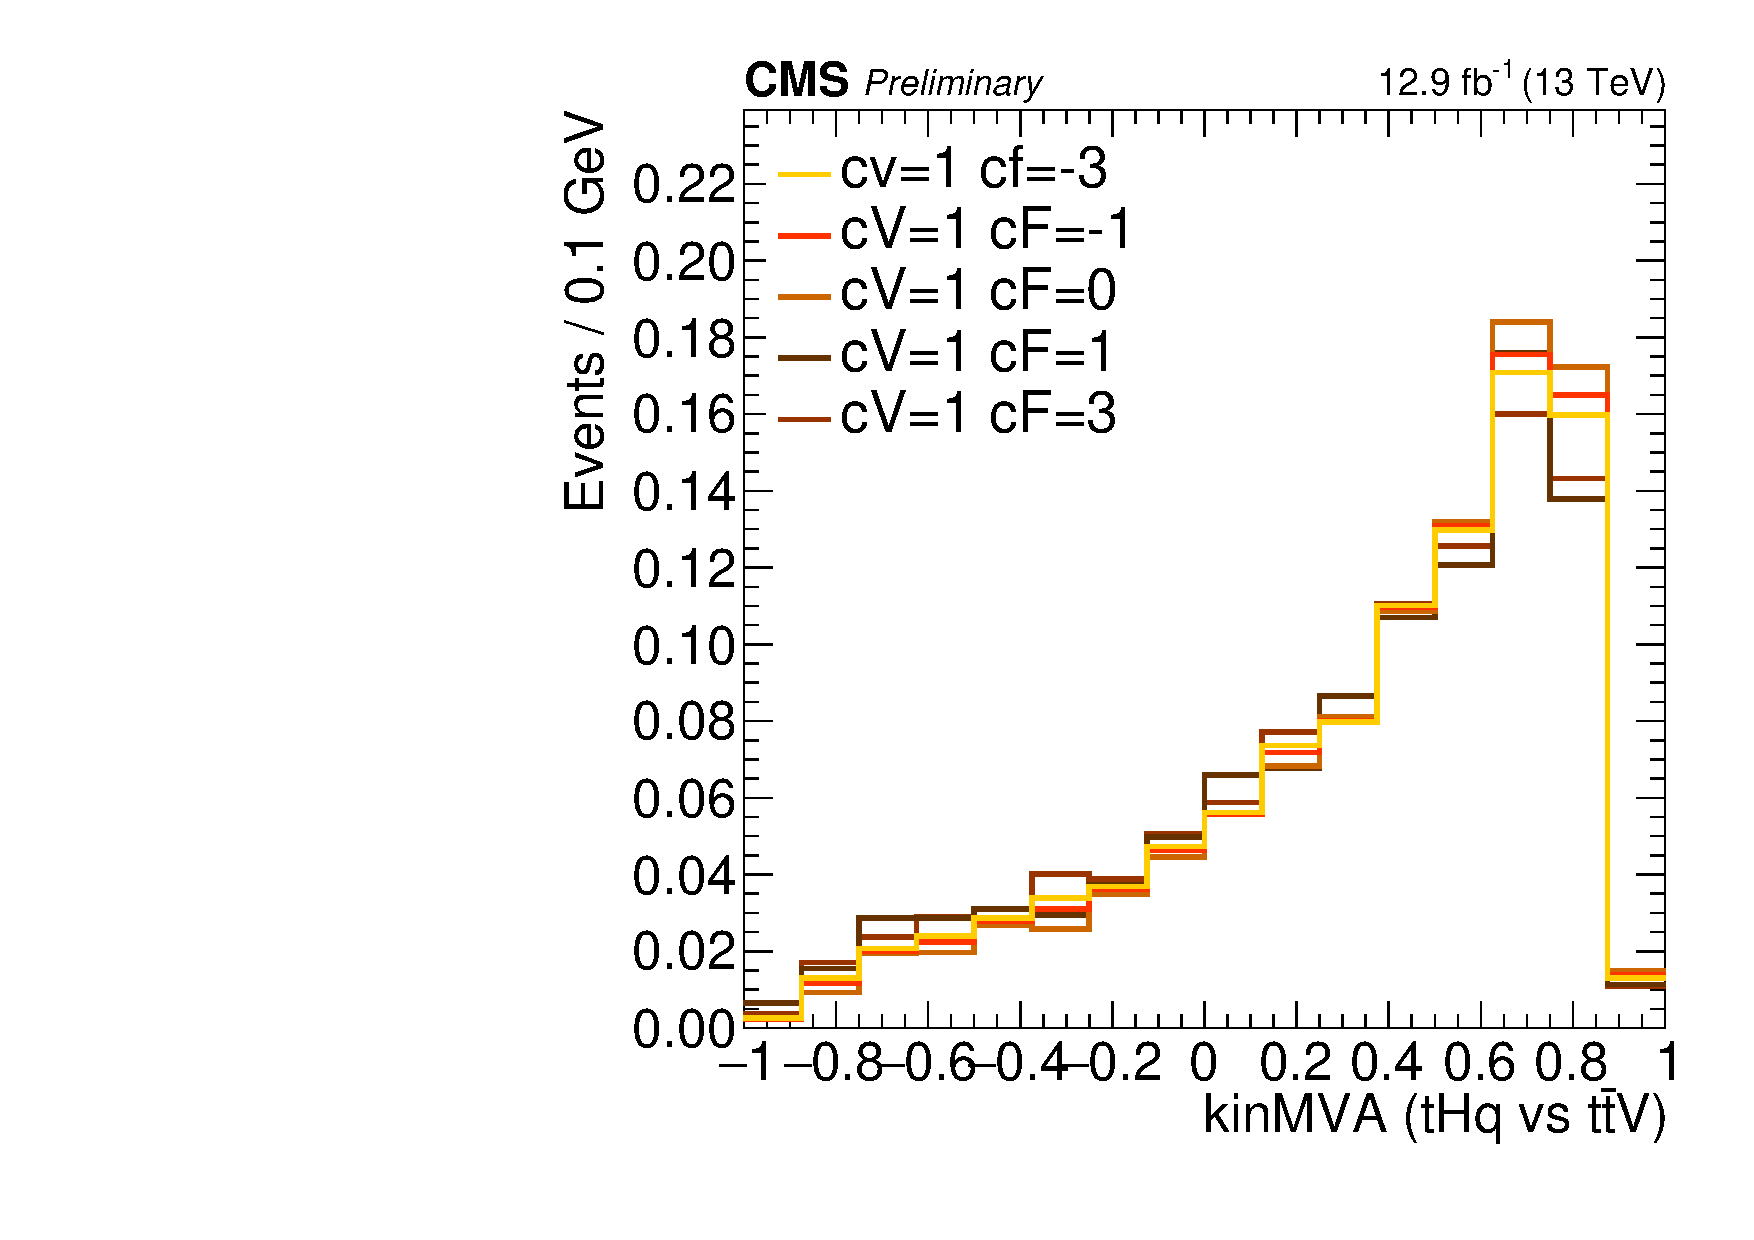
\includegraphics[width=0.45\textwidth]{figures/controlplots/bdtvscvct/thqMVA_ttv_3l.pdf}
  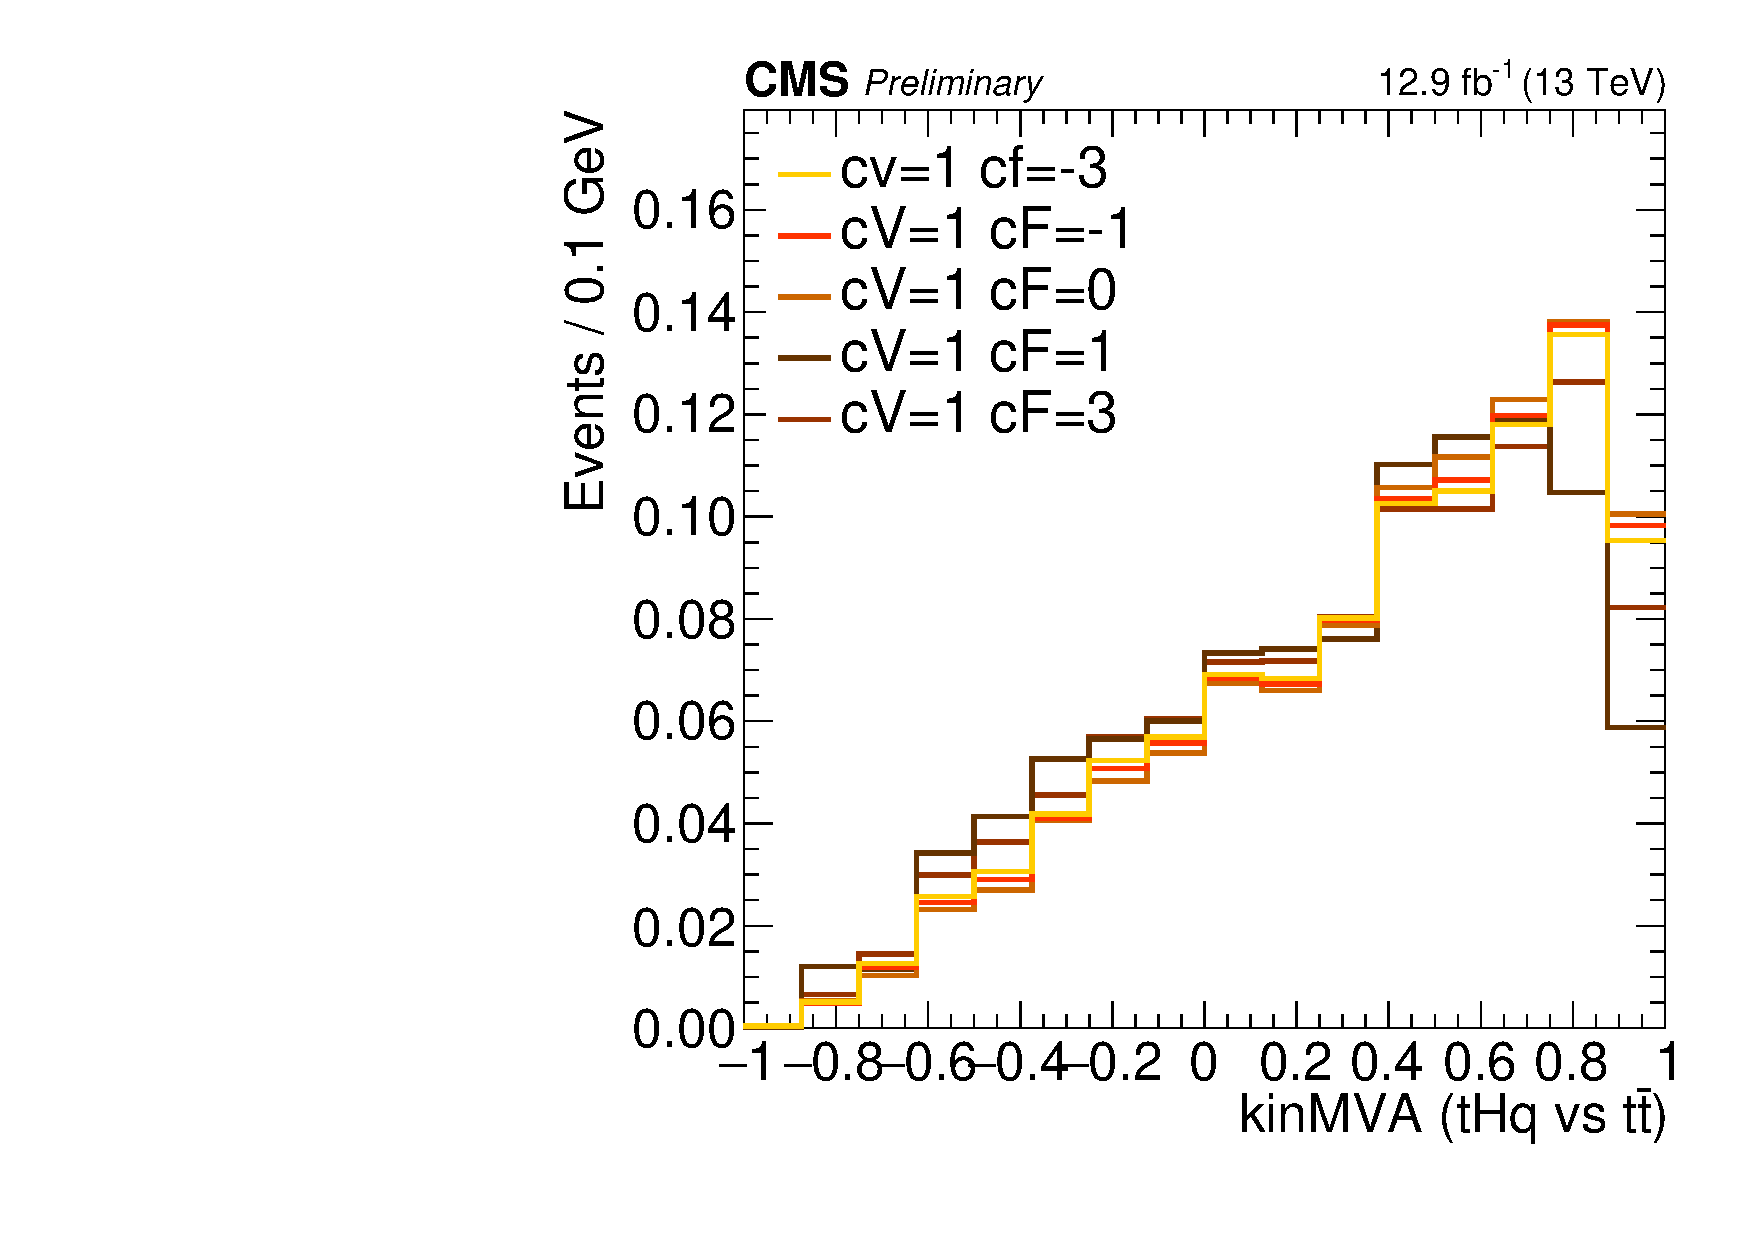
\includegraphics[width=0.45\textwidth]{figures/controlplots/bdtvscvct/thqMVA_tt_3l.pdf} \\
\caption{Change of BDT output when varying \Ct\ coupling (\CV\ is fixed at $1.0$). Training vs.\ \ttV\ (right) and vs.\ \ttbar\ (left).}
\label{fig:bdtvscvct}
\end{figure}
